\section{AFD Palabras que contienen 'web' y/o 'ebay'}
	\subsection{Descripción del problema}
	La elaboración de este programa consistió en convertir un autómata finito no determinista como el de la figura \ref{fig:diagrama1} , que reconoce las palabras 'web' y 'ebay', a un autómata finito determinista como el de la figura \ref{fig:diagrama2}.
	\begin{figure}[H]
		\begin{center}
		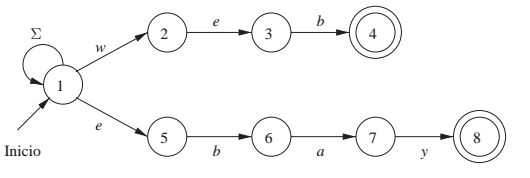
\includegraphics[width=12cm, height=4cm]{img/webay-AFND.png}
		\caption{Diagrama de un AFN que busca las palabras 'web' y 'ebay.\cite{LIBRO}}
		\label{fig:diagrama1}
		\end{center}
	\end{figure}
	Además, el programa contara con modo manual y automático, en el modo manual el usuario ingresara una cadena y se le mostrara las palabras encontradas, su posición y cuantas fueron encontradas.
	\begin{figure}[H]
		\begin{center}
			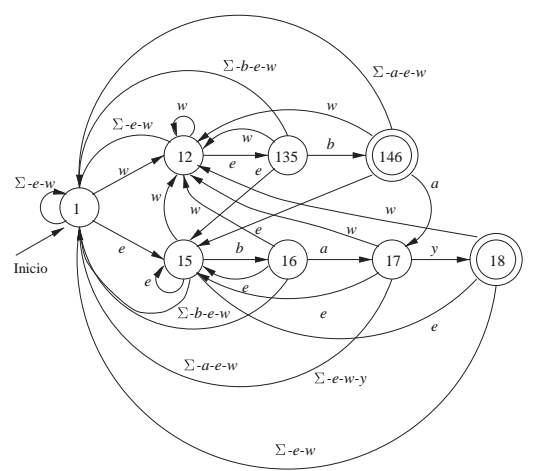
\includegraphics[width=12cm, height=10cm]{img/webay-AFD.png}
			\caption{Conversion del AFN a un AFD. \cite{LIBRO}}
			\label{fig:diagrama2}
		\end{center}
	\end{figure}
	En el modo automático se hará lo mismo pero con el agregado de que el texto se obtendrá de un archivo con extensión '.txt' y se mostrara la linea de texto en la que fue encontrada la palabra.
	Es importante señalar que todo aquello que no es un símbolo del alfabeto español, $ \sum =\lbrace a, b, ..., z, A, B, ..., Z \rbrace $, es tomado como un espacio. Además, debe tener una opción para visualizar el diagrama de la figura \ref{fig:diagrama2}.
	\subsection{Código}
	El código fue realizado en Python 3.5.
	\\Archivo: main\_webay.py
	\begin{lstlisting}[language=Python]
	# main_webay.py
	# -*- coding: utf-8 -*-
	from __future__ import print_function
	from diagrama import Diagrama
	from automata import automata

	separador = '='*50

	def main():
    continuar = True
    while continuar:
      opcion = imprimir_menu()
      if opcion == 1:
        entrada_consola()
      elif opcion == 2:
        entrada_archivo()
      elif opcion == 3:
        ver_diagrama()
      else:
        break
      print('*' * 100)
      opcion = input("Reintentar [s/n]: ")
      if opcion.lower() != 's':
        continuar = False

    print('Saliendo del programa...')

	def imprimir_menu():
    print('\n\n%sMenu%s' % (separador, separador))
    print("""
        1.- Entrada en consola
        2.- Ingresar nombre del archivo
        3.- Ver diagrama de estados
        4.- Salir
    """)
    try:
      opcion = int(input("Selecciona una opcion valida: "))
      return opcion
    except Exception as e:
      print('Error ', e)
    return 0

	def entrada_consola():
    texto = input("Escribe el texto: ")
    texto += ' '
    diccionario = {}
    diccionario = automata(texto)
    imprimir_diccionario(diccionario)

	def entrada_archivo():
    texto = input('Escribe el nombre del archivo: ')
    i = 1
    try:
      archivo = open(texto, 'r')
    except Exception as e:
      print('Error al abrir archivo: ', e)
      return 0
    diccionario = []
    num_linea = 1
    for linea in archivo:
      diccionario.append(automata(linea))
      num_linea += 1
    while i<num_linea:
      print('\nEn la linea: ', i)
      imprimir_diccionario(diccionario[i-1])
      i +=1
    archivo.close()

	def imprimir_diccionario(diccionario):
    print('\nSe encontraron %s web y %s ebays' %(diccionario['num_web'], diccionario['num_ebay']))
    print('En las posiciones:' )
    print('%s para web' %diccionario['web_pos'])
    print('%s para ebay' %diccionario['ebay_pos'])
    print('Las palabras encontradas fueron: %s' %diccionario['palabras'])

	def ver_diagrama():
    print('Mostrando diagrama del automata. Cierre la ventana para continuar')
    try:
      diagrama = Diagrama()
      diagrama.master.title('Diagrama del automata webay')
      diagrama.mainloop()
    except Exception as e:
			print("Error", e)

	main()
	\end{lstlisting}
	Archivo: automata\_webay.py
	\begin{lstlisting}[language=Python]
	# automata_webay.py
	# -*- coding: utf-8 -*-
	from __future__ import print_function

	def automata(texto):
		estado = 'B'
		palabra_aux = ''
		num_palabra = 1
		cumple = False
		ebay = 0
		palabra_posicion = 0
		ebay_pos = []
		web_pos = []
		web = 0
		palabras = []
		diccionario = {}
		for simbolo in texto:
			palabra_posicion += 1
			simbolo_aux = simbolo.lower()
			if simbolo ==  '\n':
				simbolo = '\\n'
			print('-> delta(%s,%s)' % (estado, simbolo), end="\t")
			estado = estados(estado, simbolo_aux)
			if estado == 'G' or estado == 'I':
				cumple = True
			if estado == 'G':
				web += 1
				web_pos.append([palabra_posicion-2, palabra_posicion])
			elif estado == 'I':
				ebay += 1
				ebay_pos.append([palabra_posicion-3, palabra_posicion])

			if ((ord(simbolo_aux) < 123 and ord(simbolo_aux) > 96) or ord(simbolo_aux) == 241):
				palabra_aux += simbolo
			else:
				if cumple:
					palabras.append(palabra_aux)
					cumple = False
				palabra_aux = ''
		diccionario = {'num_web': web, 'num_ebay':ebay, 'web_pos':web_pos, 'ebay_pos':ebay_pos, 'palabras':palabras}
		return diccionario

	def estados(estado, simbolo):
		if estado == 'B':
			estado = estado_B(simbolo)
		elif estado == 'C':
			estado = estado_C(simbolo)
		elif estado == 'D':
			estado = estado_D(simbolo)
		elif estado == 'E':
			estado = estado_E(simbolo)
		elif estado == 'F':
			estado = estado_F(simbolo)
		elif estado == 'G':
			estado = estado_G(simbolo)
		elif estado == 'H':
			estado = estado_H(simbolo)
		elif estado == 'I':
			estado = estado_I(simbolo)
		else:
			estado = 'A'

		return estado

	def estado_B(simbolo):
		if simbolo == 'w':
			return 'C'
		elif simbolo == 'e':
			return 'D'
		return 'B'

	def estado_C(simbolo):
		if simbolo == 'w':
			return 'C'
		elif simbolo == 'e':
			return 'E'
		return 'B'

	def estado_D(simbolo):
		if simbolo == 'b':
			return 'F'
		elif simbolo == 'e':
			return 'D'
		elif simbolo == 'w':
			return 'C'
		return 'B'

	def estado_E(simbolo):
		if simbolo == 'b':
			return 'G'
		elif simbolo == 'e':
			return 'D'
		elif simbolo == 'w':
			return 'C'
		return 'B'

	def estado_F(simbolo):
		if simbolo == 'a':
			return 'H'
		elif simbolo == 'e':
			return 'D'
		elif simbolo == 'w':
			return 'C'
		return 'B'

	def estado_G(simbolo):
		if simbolo == 'a':
			return 'H'
		elif simbolo == 'e':
			return 'D'
		elif simbolo == 'w':
			return 'C'
		return 'B'

	def estado_H(simbolo):
		if simbolo == 'y':
			return 'I'
		elif simbolo == 'e':
			return 'D'
		elif simbolo == 'w':
			return 'C'
		return 'B'

	def estado_I(simbolo):
		if simbolo == 'e':
			return 'D'
		elif simbolo == 'w':
			return 'C'
		return 'B'
	\end{lstlisting}
	Archivo: diagrama\_webay.py
	\begin{lstlisting}[language=Python]
	# diagrama_webay.py
	# -*- coding: utf-8 -*-
	from __future__ import print_function
	import tkinter as tk

	class Diagrama(tk.Frame):
	    def __init__(self, master=None):
	        super().__init__(master, background='white')
	        self.pack(fill=tk.BOTH, expand=tk.YES)
	        self.canvas = tk.Canvas(self, bg='white')
	        self.canvas.pack(fill=tk.BOTH, expand=1)
	        self.dibujarDiagrama()
	        self.centrarVentana()

	    def dibujarDiagrama(self):
	        coord_circulo = [100, 205, 150, 255]
	        self.dibujarLinea([25, 275, 100, 275])
	        self.dibujarCirculo([100, 255, 150, 305])
	        self.dibujar_bases()
	        self.reflexiva()
	        self.normal()
	        self.reves()
	        self.masflechas()
	        self.puntos()
	        self.letras()
	        self.etiquetas()

	    def etiquetas(self):
	        self.canvas.create_text(75, 245, text='S-e-w')
	        self.canvas.create_text(150, 180, text='S-e-w')
	        self.canvas.create_text(405, 565, text='S-e-w')
	        self.canvas.create_text(260, 465, text='S-a-e-w')
	        self.canvas.create_text(515, 90, text='S-a-e-w')
	        self.canvas.create_text(180, 400, text='S-b-e-w')
	        self.canvas.create_text(300, 90, text='S-b-e-w')
	        self.canvas.create_text(380, 530, text='S-e-w-y')
	        self.canvas.create_text(500, 510, text='e')
	        self.canvas.create_text(400, 460, text='e')
	        self.canvas.create_text(300, 420, text='e')
	        self.canvas.create_text(210, 325, text='e')
	        self.canvas.create_text(180, 335, text='e')
	        self.canvas.create_text(300, 170, text='e')
	        self.canvas.create_text(355, 215, text='e')
	        self.canvas.create_text(480, 230, text='e')
	        self.canvas.create_text(600, 310, text='w')
	        self.canvas.create_text(500, 320, text='w')
	        self.canvas.create_text(450, 100, text='w')
	        self.canvas.create_text(310, 140, text='w')
	        self.canvas.create_text(220, 130, text='w')
	        self.canvas.create_text(165, 215, text='w')
	        self.canvas.create_text(220, 235, text='w')
	        self.canvas.create_text(280, 255, text='w')
	        self.canvas.create_text(470, 170, text='b')
	        self.canvas.create_text(305, 370, text='b')
	        self.canvas.create_text(605, 370, text='y')

	        self.canvas.create_text(455, 370, text='a')
	        self.canvas.create_text(555, 250, text='a')

	    def letras(self):
	        self.canvas.create_text(50, 265, text='Inicio')
	        self.canvas.create_text(125, 150+130, text='B')
	        self.canvas.create_text(225, 100+80, text='C')
	        self.canvas.create_text(385, 100+80, text='E')
	        self.canvas.create_text(545, 100+80, text='G')
	        self.canvas.create_text(225, 250+130, text='D')
	        self.canvas.create_text(385, 250+130, text='F')
	        self.canvas.create_text(545, 250+130, text='H')
	        self.canvas.create_text(705, 250+130, text='I')

	    def dibujarCirculo(self, coordenadas):
	        self.canvas.create_oval(coordenadas)

	    def dibujarLinea(self, coord):
	        self.canvas.create_line(coord)
	        self.canvas.create_oval(coord[2]-3, coord[3]-3, coord[2]+3, coord[3]+3, fill='black')

	    def dibujar_bases(self):
	        x, y = 100, 100
	        for num in range(3):
	            self.dibujarLinea([140, 260, 200, 185])
	            self.dibujarCirculo([100+x, 255-y, 150+x, 305-y])
	            self.dibujarLinea([250, 180, 360, 180])
	            self.dibujarLinea([410, 180, 520, 180])
	            self.dibujarLinea([140, 300, 200, 380])
	            self.dibujarCirculo([100+x, 255+y, 150+x, 305+y])
	            self.dibujarLinea([150+x, 380, 260+x, 380])
	            x = x + 160
	            if num == 2:
	                self.dibujarCirculo([100+x, 255+y, 150+x, 305+y])
	                self.dibujarCirculo([105+x, 260+y, 145+x, 300+y])
	                self.dibujarCirculo([105+x-160, 260-y, 145+x-160, 300-y])

	    def reflexiva(self):
	        extra = {'start': 20, 'extend': 255}
	        self.crear_arco([85, 245, 120, 275], extra)
	        extra = {'start': -20, 'extend': 275}
	        self.crear_arco([195, 135, 225, 165], extra)
	        extra = {'start': -20, 'extend': 275}
	        self.crear_arco([195, 335, 225, 365], extra)

	    def normal(self):
	        extra = {'start': 87, 'extend': 105}
	        self.crear_arco([125, 175, 270, 310], extra)
	        extra = {'start': 45, 'extend': 95}
	        self.crear_arco([225, 150, 390, 250], extra)
	        extra = {'start': 25, 'extend': 135}
	        self.crear_arco([235, 105, 545, 300], extra)
	        extra = {'start': 30, 'extend': 165}
	        self.crear_arco([120, 100, 385, 350], extra)
	        extra = {'start': 20, 'extend': 150}
	        self.crear_arco([120, 25, 545, 450], extra)

	    def reves(self):
	        extra = {'start': -87, 'extend': -105}
	        self.crear_arco([125, 250, 270, 390], extra)
	        extra = {'start': -45, 'extend': -95}
	        self.crear_arco([225, 310, 390, 410], extra)
	        extra = {'start': -25, 'extend': -135}
	        self.crear_arco([235, 260, 545, 455], extra)
	        extra = {'start': -30, 'extend': -160}
	        self.crear_arco([125, 205, 385, 455], extra)
	        extra = {'start': -24, 'extend': -150}
	        self.crear_arco([123, 115, 550, 520], extra)
	        extra = {'start': -20, 'extend': -150}
	        self.crear_arco([123, 50, 730, 580], extra)
	        extra = {'start': -20, 'extend': -145}
	        self.crear_arco([235, 200, 730, 500], extra)

	    def masflechas(self):
	        self.dibujarLinea([545, 205, 555, 355])

	        self.dibujarLinea([545, 355, 235, 200])
	        self.dibujarLinea([700, 355, 235, 200])
	        self.dibujarLinea([385, 355, 235, 200])
	        self.dibujarLinea([545, 205, 240, 360])
	        self.dibujarLinea([385, 205, 240, 360])
	        self.dibujarLinea([230, 355,235, 200])

	    def crear_arco(self, coord, extra=None):
	        self.canvas.create_arc(coord, start=extra['start'], extent=extra['extend'], style='arc')

	    def puntos(self):
	        self.canvas.create_oval(123, 250, 129, 257, fill='black')
	        self.canvas.create_oval(124, 301, 131, 308, fill='black')
	        self.canvas.create_oval(204, 361, 211, 368, fill='black')
	        self.canvas.create_oval(242, 389, 249, 396, fill='black')
	        self.canvas.create_oval(204, 161, 211, 168, fill='black')

	        self.canvas.create_oval(242, 163, 249, 170, fill='black')

	    def centrarVentana(self):
	        ancho, altura = 850, 605
	        ancho_pantalla = self.winfo_screenwidth()
	        altura_pantalla = self.winfo_screenheight()
	        posicion_x = (ancho_pantalla - ancho)/2
	        posicion_y = (altura_pantalla - altura)/2
	        self.master.geometry('%dx%d+%d+%d' % (ancho, altura, posicion_x, posicion_y))

	\end{lstlisting}
	\subsection{Pruebas}
	Pruebas de las opciones del menú.
	\\
	{\large Modo de manual.}
	\begin{figure}[H]
		\begin{center}
			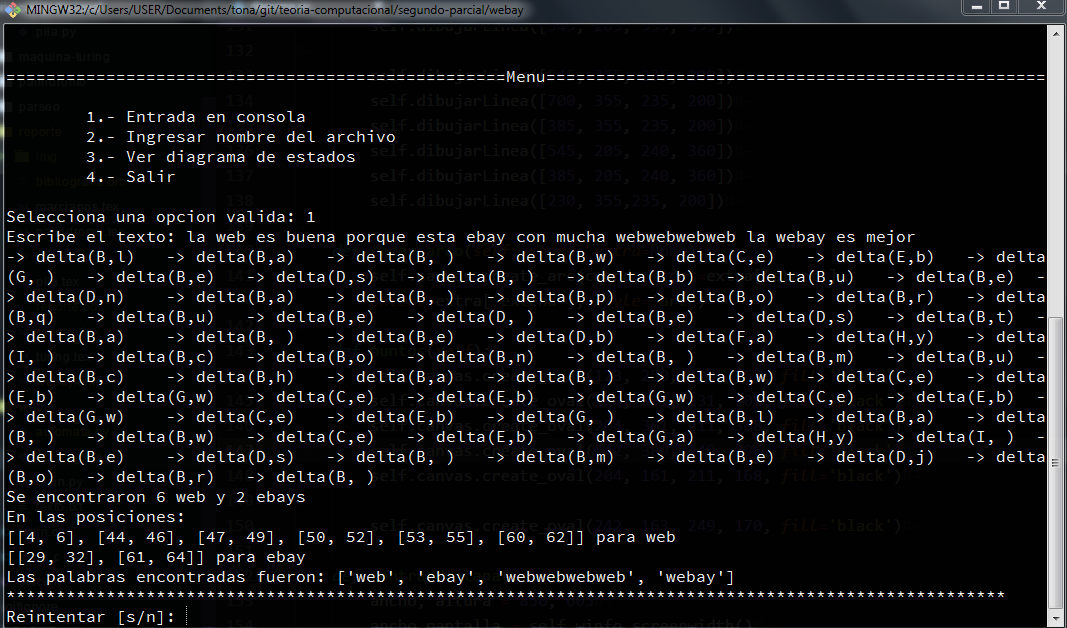
\includegraphics[width=\linewidth, height=10cm]{img/webay-manual.png}
			\caption{Historia del autómata y las palabras con 'web' y/o 'ebay'.}
			\label{fig:webay1}
		\end{center}
	\end{figure}
	\newpage
	{\large Modo automático}
	\begin{figure}[H]
		\begin{center}
			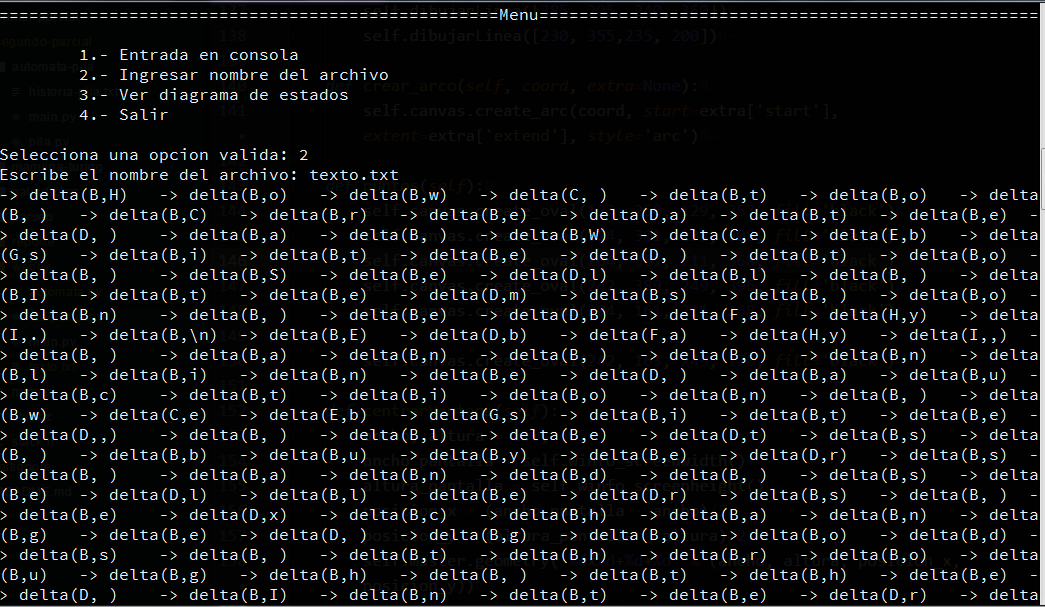
\includegraphics[width=\linewidth, height=9cm]{img/webay-automatico1.png}
			\caption{Parte de la historia del autómata y las palabras con 'web' y/o 'ebay'.}
			\label{fig:webay2}
		\end{center}
	\end{figure}
\begin{figure}[H]
	\begin{center}
		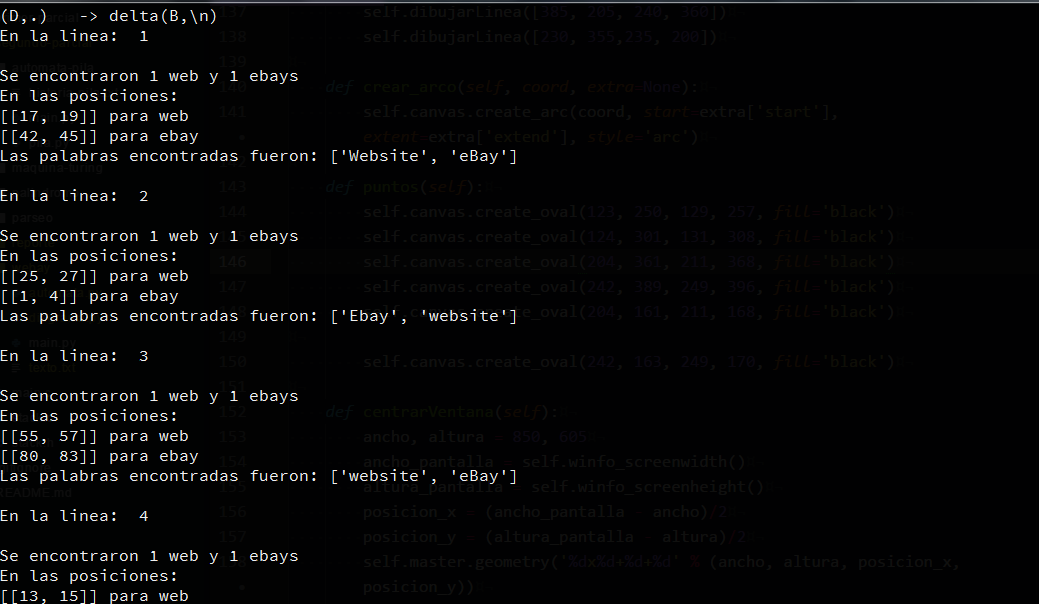
\includegraphics[width=\linewidth, height=9cm]{img/webay-automatico2.png}
		\caption{Parte de la historia del autómata y las palabras con 'web' y/o 'ebay'.}
		\label{fig:webay3}
	\end{center}
\end{figure}
	{\large Diagrama.}
	\begin{figure}[H]
		\begin{center}
			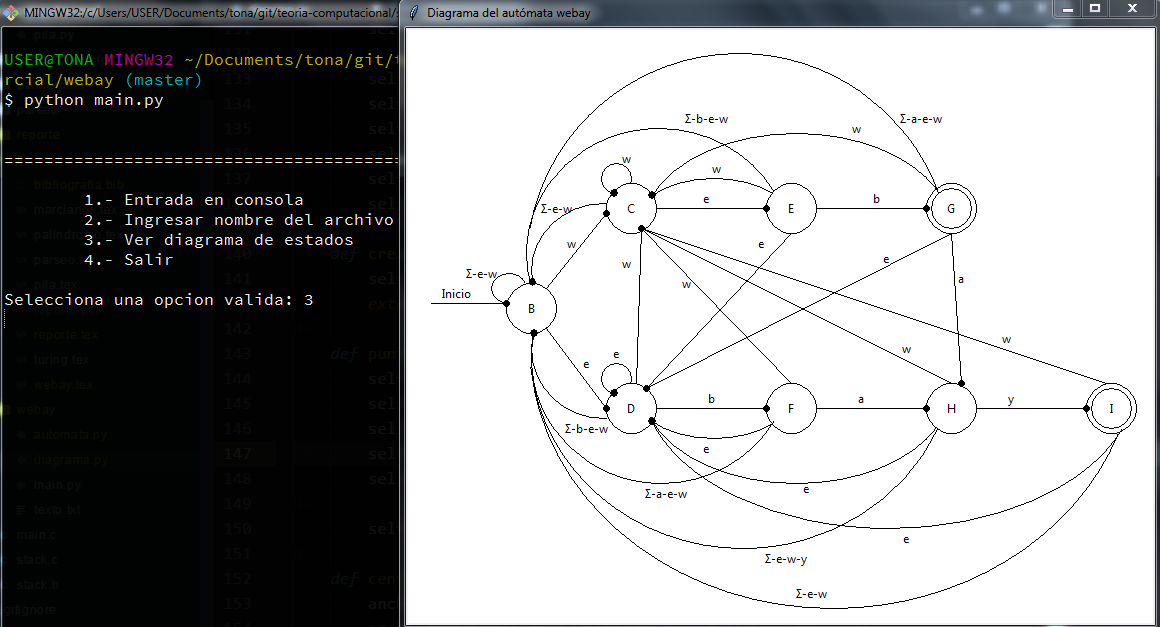
\includegraphics[width=\linewidth, height=9cm]{img/webay-diagrama.png}
			\caption{Diagrama de transiciones del autómata 'webay'.}
			\label{fig:webay4}
		\end{center}
	\end{figure}
